\section{Introduction}\label{sec:introduction}

If you are new to \LaTeX{}, you can check my YouTube video \href{https://youtu.be/CjuYkcA35dw}{\LaTeX{} Masterclass}.

If you are in a hurry, you can check my YouTube video \href{https://youtu.be/g0YdIs4oJm8}{Introduction to \LaTeX{}}.

\subsection{How to cite a paper}\label{subsec:how-to-cite-a-paper}
This is an example on how to cite a paper~\cite{Tartarini2020a}.

\subsection{How to add acronyms/nomenclature}\label{subsec:how-to-add-acronyms}
This is an example on how to add acronyms.
You can reference the acronym using the command \verb!\ac{t-db}! this will result in the following \ac{t-db}.
If you use the command \verb!\ac{t-db}! again, it will result in \ac{t-db}.
You can check the list of acronyms in the \texttt{myacronyms.tex} file.

\subsection{Glossary}\label{subsec:glossary}

This is an example on how to add a glossary.
You can reference the glossary using the command \verb!\gls{7730}! this will result in the following \gls{7730}.
You can check the list of glossary terms in the \texttt{myglossary.tex} file.

\subsection{How to add a table}\label{subsec:how-to-add-a-table}
This is an example on how to add a table.
The table is shown in Table~\ref{tab:example}.

\begin{table}[htb!]
    \centering
    \begin{tabular}{|c|c|}
        \hline
        \textbf{Column 1} & \textbf{Column 2} \\
        \hline
        Row 1 & Value 1 \\
        Row 2 & Value 2 \\
        Row 3 & Value 3 \\
        \hline
    \end{tabular}
    \caption{This is an example table.}
    \label{tab:example}
\end{table}

\subsection{How to add a figure}\label{subsec:how-to-add-a-figure}
This is an example on how to add a figure.
The figure is shown in Figure~\ref{fig:example}.

\begin{figure}[htb!]
    \centering
    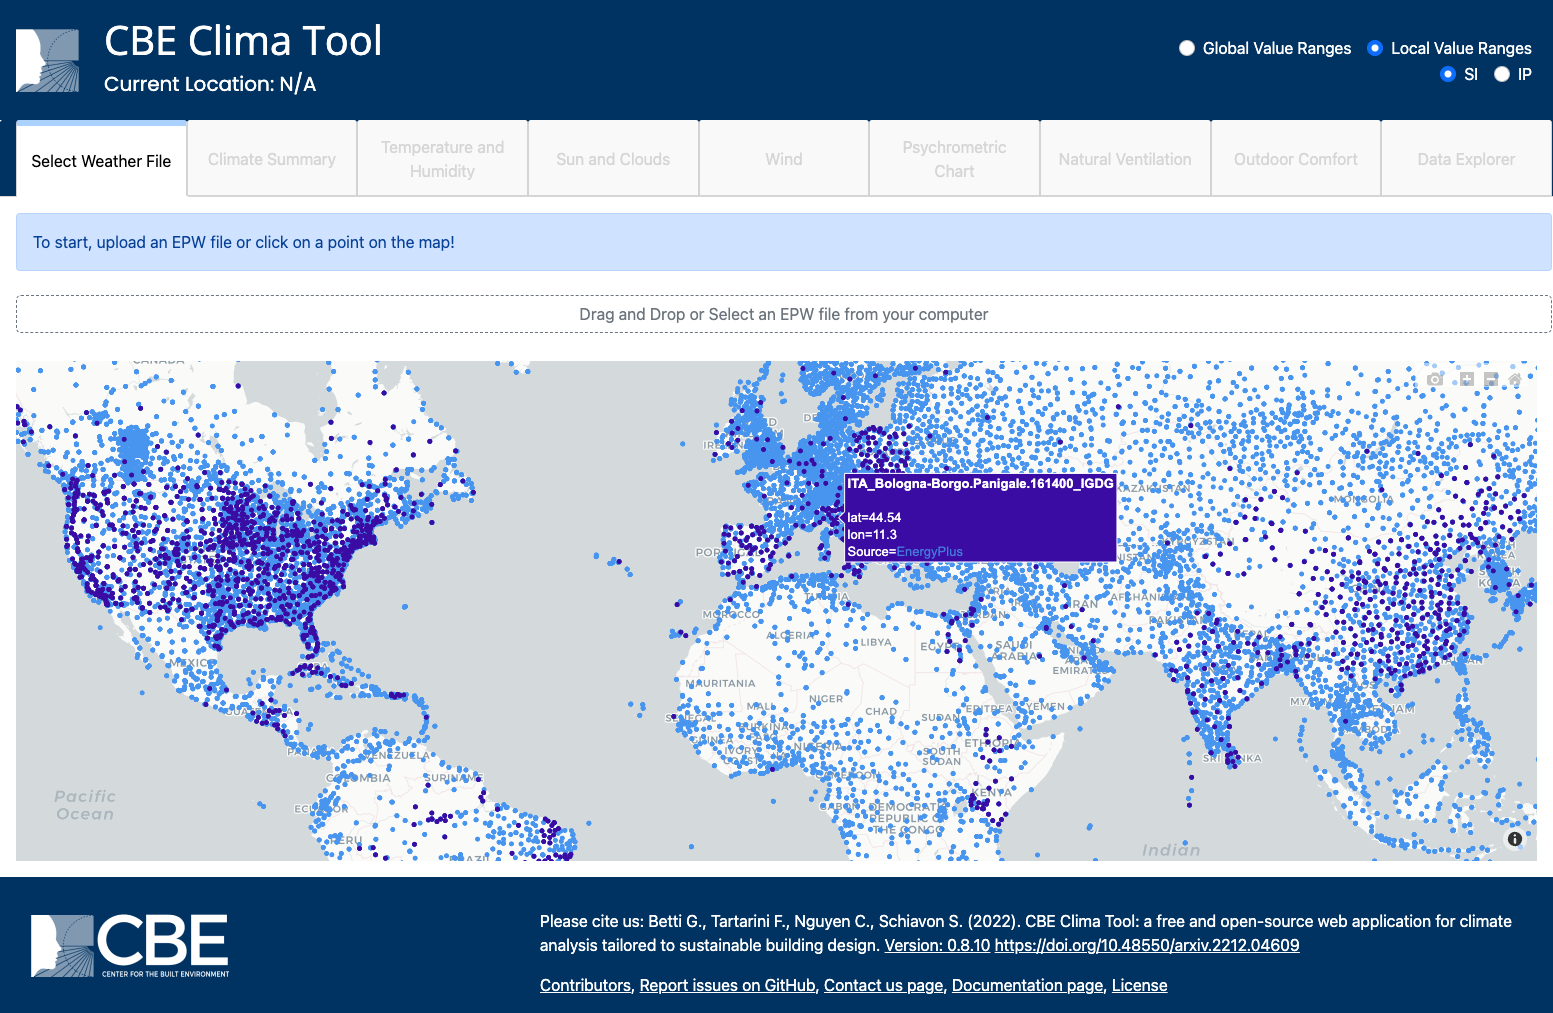
\includegraphics[width=0.75\textwidth]{figures/example_clima}
    \caption{This is an example figure.}
    \label{fig:example}
\end{figure}

\subsection{How to write numbers}\label{subsec:how-to-write-numbers}
This is an example on how to write numbers.
You can write numbers in text using the command \verb!\num{1000}! this will result in the following \num{1000}.
You can write quantities using the command \verb!\qty{1000}{\m\per\s}! this will result in \qty{1000}{\m\per\s}.

\subsection{How to import a variable}\label{subsec:how-to-import-a-variable}
This is an example on how to import a variable.
You can import a variable using the command \verb!\var{example_variable}! this will result in the following \var{example_variable}.
You can check the list of variables in the \texttt{mydata.tex} file.
If you want to find out more on how to import variables, you can check my YouTube video \href{https://ctan.org/pkg/datatool}{datatool} package documentation.